\documentclass{report}
\usepackage[margin=1in, paperwidth=8.5in, paperheight=11in]{geometry}
%Math packages%
\usepackage{amsmath}
\usepackage{amsthm}
%Spacing%
\usepackage{setspace}
\onehalfspacing
%Lecture number%
\newcommand{\lectureNum}{19}
%Variables - Date and Course%
\newcommand{\curDate}{March 14, 2017}
\newcommand{\course}{CS 241}
\newcommand{\instructor}{Kevin Lanctot}
%Defining the example tag%
%\theoremstyle{definition}%
\newtheorem{ex}{Example}[section]
%Setting counter given the lecture number%
\setcounter{chapter}{\lectureNum{}}
%Package to insert code%
\usepackage{listings}
\usepackage{courier}
\usepackage{xcolor}
\lstset { %
    tabsize=2,
    breaklines=true,
    language=C++,
    backgroundcolor=\color{blue!8}, % set backgroundcolor
    basicstyle=\footnotesize\ttfamily,% basic font setting
}
%Package for images%
\usepackage{graphicx}

\begin{document}
%Note title%
\begin{center}
\begin{Large}
\textsc{\course{} | Lecture \lectureNum{}}
\end{Large}
\end{center} 
\noindent \textit{Bartosz Antczak} \hfill
\textit{Instructor: \instructor{}} \hfill
\textit{\curDate{}}
\rule{\textwidth}{0.4pt}
% Actual Notes%
\section{Code Generation}
Once we scan the program and have our parse tree, we want to generate the actual MIPS assembly language. We'll choose MIPS code that is simplest to use, especially for CS 241 students. We'll translate the syntax from our parse tree into code using \textit{Syntax-directed Translation}.
\subsection{Overview}
Given a parse tree, we generate code for a given node in the tree by first generating the code for the node's children. We then bring all of the children's code together and there we have it | the current node's code.
\begin{figure}[ht]
\begin{center}
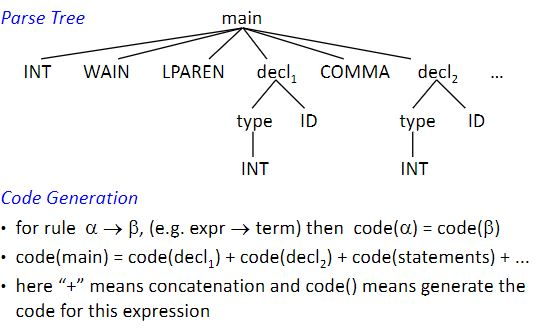
\includegraphics[scale=0.6]{code_gen.jpg}
\end{center}
\caption{\textit{Courtesy of Prof. Lanctot's slides.}}
\end{figure}
\subsection{Storing Variables (A9P1)}
\begin{ex}
\end{ex}
\noindent \texttt{int wain(int a, int b) \{ return a; \}}
\subsubsection{Output}
\texttt{add \$3, \$1, \$0}\\
\texttt{jr \$31}
\subsubsection{Conventions}
We say that \$1 and \$2 hold the parameters for the \texttt{wain} function. \$3 holds the return value.
\begin{ex}
\end{ex}
\noindent \texttt{int wain(int a, int b) \{ return b; \}}
\subsubsection{Output}
\texttt{add \$3, \$2, \$0}\\
\texttt{jr \$31}
\subsubsection{Observations}
Both of these examples have the same parse tree, so how do we differentiate the programs? We add a Location column to our Symbol Table:
\begin{figure}[ht]
\begin{center}
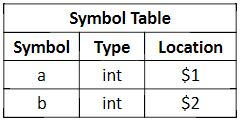
\includegraphics[scale=0.6]{symb.jpg}
\end{center}
\caption{\textit{Courtesy of Prof. Lanctot's slides.}}
\end{figure}
\subsection{Methods of Storing Variables}
We can use a \textbf{stack}, where each variable's location is determined on their position in the stack. An example is shown:
\begin{figure}[ht]
\begin{center}
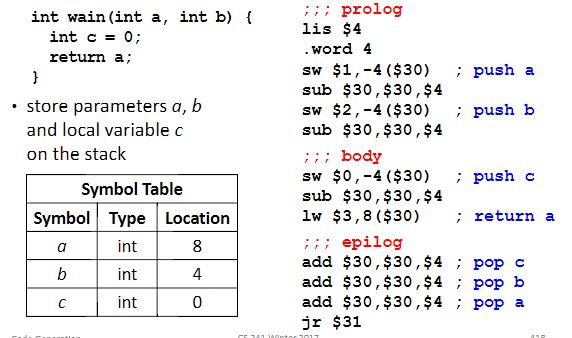
\includegraphics[scale=0.6]{stack.jpg}
\end{center}
\caption{\textit{Courtesy of Prof. Lanctot's slides.}}
\end{figure}
\subsubsection{A Problem Arises}
We don't know the offsets to the parameters and variables until all the variables (for that function) have been defined.\newpage
The \textbf{solution} is to include a frame pointer. We reserve \$29 to point to the first element of the stack, and any offsets in the symbol table will be relative to the frame pointer. An example utilizing this solution is shown:
\begin{figure}[ht]
\begin{center}
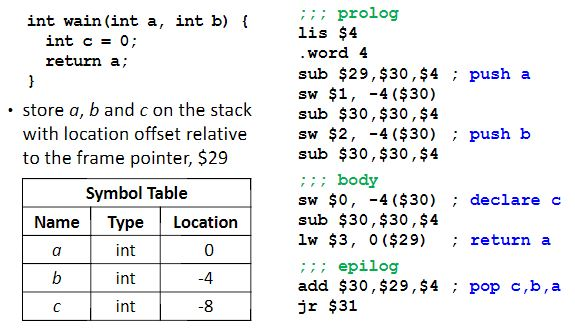
\includegraphics[scale=0.6]{symb2.jpg}
\end{center}
\caption{The variable's location are in reference to the frame pointer. See that $a$ is zero away from the frame pointer, $b$ is -4 away, and so on. \textit{Courtesy of Prof. Lanctot's slides.}}
\end{figure}
\subsection{Some Conventions for Code Generation (for CS 241)}
\begin{itemize}
\item \textbf{\$0:} always 0 (or false)
\item \textbf{\$1:} value of first parameter / argument
\item \textbf{\$2:} value of second parameter / argument
\item \textbf{\$3:} result of calculations
\item \textbf{\$4:} constant 4 (helpful for pushing on and popping off stack)
\item \textbf{\$5:} store previous intermediate results
\item \textbf{\$11:} always 1
\item \textbf{\$29:} frame pointer (fp)
\item \textbf{\$30:} stack pointer (sp)
\item \textbf{\$31:} return address (ra)
\end{itemize}
\subsubsection{Structuring our MIPS Code}
It will be subdivided into three sections:
\begin{itemize}
\item \textbf{Prologue}: push return address and arguments on stack
\item \textbf{Generated Code}: put local variables on stack and generate code for body of function
\item \textbf{Epilogue}: pop local variables and arguments off stack; restore previous return address to \$310
\end{itemize}
\subsection{Some Examples of Code Generation}
\begin{ex}
A9P2:
\end{ex}
Here, we simply ignore the parentheses since they don't generate any code. We simply evaluate the expression in it:
\begin{figure}[ht]
\begin{center}
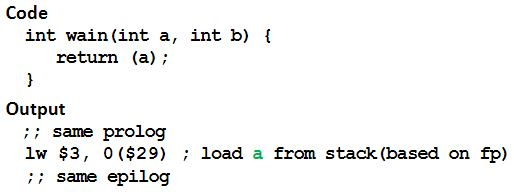
\includegraphics[scale=0.6]{a9p2.jpg}
\end{center}
\caption{\textit{Courtesy of Prof. Lanctot's slides.}}
\end{figure}
\begin{ex}
A9P3:
\end{ex}
\begin{figure}[ht]
\begin{center}
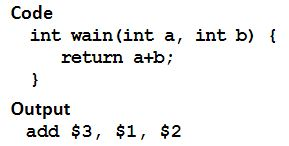
\includegraphics[scale=0.5]{a9p3.jpg}
\end{center}
\caption{\textit{Courtesy of Prof. Lanctot's slides.}}
\end{figure}
How we we deal with general expressions? (e.g., $a+b+c+d+e+\cdots$)
\subsubsection{Solution}
We use our special registers \$3 and \$5!
For the rule $expr_1 \rightarrow expr_2 + term$, we perform the following:
\begin{itemize}
\item Evaluate $expr_2$ and store in \$3
\item Push the value of \$3 onto the stack
\item Now evaluate $term$ and overwrite it into \$3
\item Pop the value of $expr_2$ off the stack and store in \$5
\item Add \$5 and \$3 together and store in \$3
\end{itemize}
\begin{figure}[ht]
\begin{center}
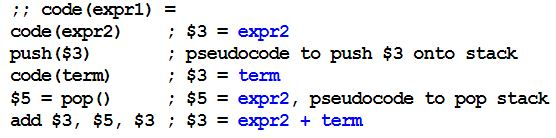
\includegraphics[scale=0.5]{a9p3-2.jpg}
\end{center}
\caption{Pseudo code of the approach. \textit{Courtesy of Prof. Lanctot's slides.}}
\end{figure}
\begin{ex}
A9P4
\end{ex}
For rule $statements \rightarrow PRINTLN \,\, LPAREN \,\,expr\,\, RPARENT$, we perform a function call to \texttt{print}, which will be provided for us (yes!). We must import \texttt{print} in our MIPS language:
\begin{itemize}
\item First compile your wlp4i code into assembly
\item Then convert your assembly file to a merl file
\item Finally, link said merl file with \texttt{print.merl} and output the file into your executable merl file
\end{itemize}
\begin{figure}[ht]
\begin{center}
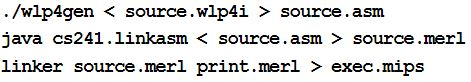
\includegraphics[scale=0.7]{linker.jpg}
\end{center}
\caption{\textit{Courtesy of Prof. Lanctot's slides.}}
\end{figure}
\textbf{Note:} the \texttt{print} file overwrites whatever content is in \$1 and \$31. \$1 is okay to be overwritten, but we need to store whatever is in \$31 onto the stack. Once we finish our code, in our epilogue, we pop the value off the stack and restore it into \$31.
%END%
\end{document}